\subsection{Computation of derivatives}
\label{sec:derivatives}

Computation of derivative quantities such as gradient and Laplacian is of fundamental importance in
data analysis. In this section, we study streams that aim to minimize errors of derivative fields.
For the experiments in this section, we quantize the data to $32$ instead of $16$ bits, to ensure
enough precision for the purpose of taking derivatives using finite differences of floating-point
values. Note that in this paper, for the purpose of derivative computation, we always perform finite
differences on the finest (original) resolution. This is possible since the wavelet transform allows
for reconstruction of the function at the original resolution. The reason for this decision is to
avoid the problem of computing distances between quantities across grids of different dimensions
(e.g., computing the root-mean-square error between a (down-sampled) $n\times n$ grid and a
$2n\times 2n$ grid), because we are unaware of widely accepted solutions to this problem. In the
following sections, we perform experiments with two of the most common types of derivative, namely
gradient (Section~\ref{sec:gradient}) and Laplacian (Section~\ref{sec:laplacian}).

\subsubsection{Gradient}
\label{sec:gradient}

Since simulation data can rarely be captured by closed-form formulas, we use finite difference to
compute gradients. We experiment with three popular finite difference schemes using stencil size
widths of two, three, and five points in each dimension, but found no tangible differences in the
results. We have therefore decided to use the five-point stencil exlusively in this paper:
$\frac{\partial f}{\partial x}\approx
\frac{1}{12}f(x-2)-\frac{2}{3}f(x-1)+\frac{2}{3}f(x+1)-\frac{1}{12}f(x+2)$. In 2D, the gradient at
each grid point $(x,y)$ is the vector $(\frac{\partial f}{\partial x},\frac{\partial f}{\partial
y})$. We use Algorithm~\ref{alg:greedy} to compute a \emph{gradient-optimized} stream that minimizes
the difference between the gradient field of $f_b$ (the reconstructed function using $b$ bits per
sample) and that of the original function ($f$). At each grid point $p$, we compute an error $e(p)$,
defined to be the squared Euclidean length of the difference between two gradient vectors at $p$,
that is $e(p)=\norm{\nabla f_b(p)-\nabla f(p)}^2$. The overall error metric over the whole field,
$E_g$, is defined as $E_g(\nabla f_b,\nabla f)=\sqrt{\frac{1}{n}\sum_{i=1}^{n}{e(p_i)}}$.

We plot the gradient error curves produced by the \emph{by level}, \emph{by bit plane}, \emph{by
wavelet norm}, \emph{gradient-optimized}, and \emph{gradient signature} streams, for six data sets
(Figure~\ref{fig:gradient-error-comparison}). \emph{gradient-optimized} performs far better than all
the static streams, due to the fact that, with the knowledge of the data, this stream is able to
prioritize regions that would benefit the most from additional bits. Among the static streams,
\emph{by level} performs the worst, while \emph{by wavelet norm} performs slightly worse than the
other two streams. 

\begin{figure}[h]
	\centering
	\subcaptionbox{boiler}{
	{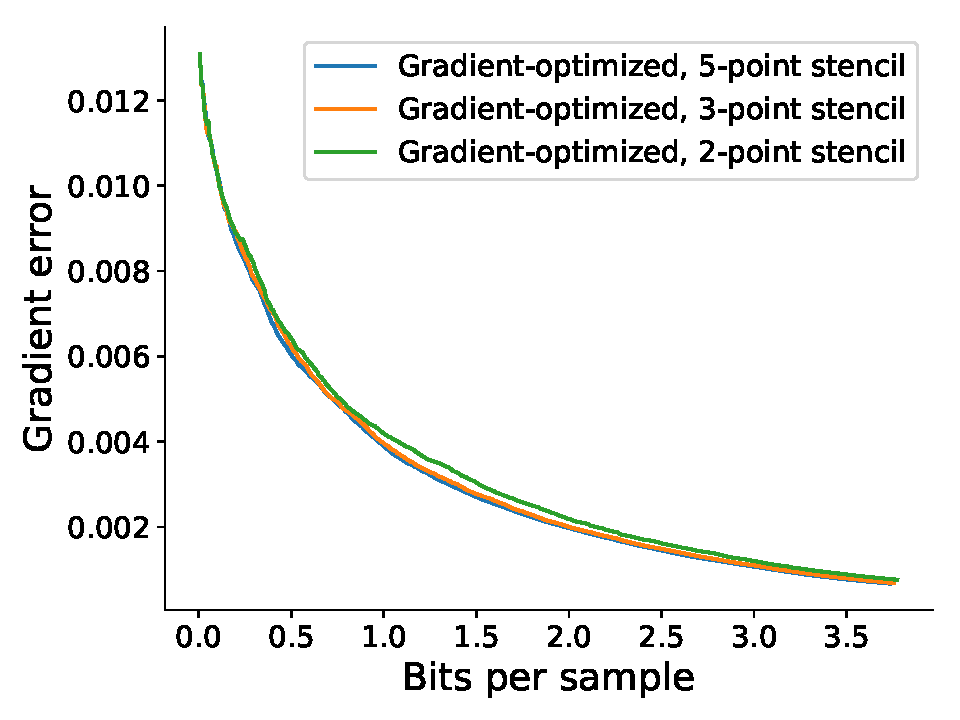
\includegraphics[width=0.48\linewidth]{gradient/gradient-optimized-boiler}}}
	\subcaptionbox{diffusivity}{
	{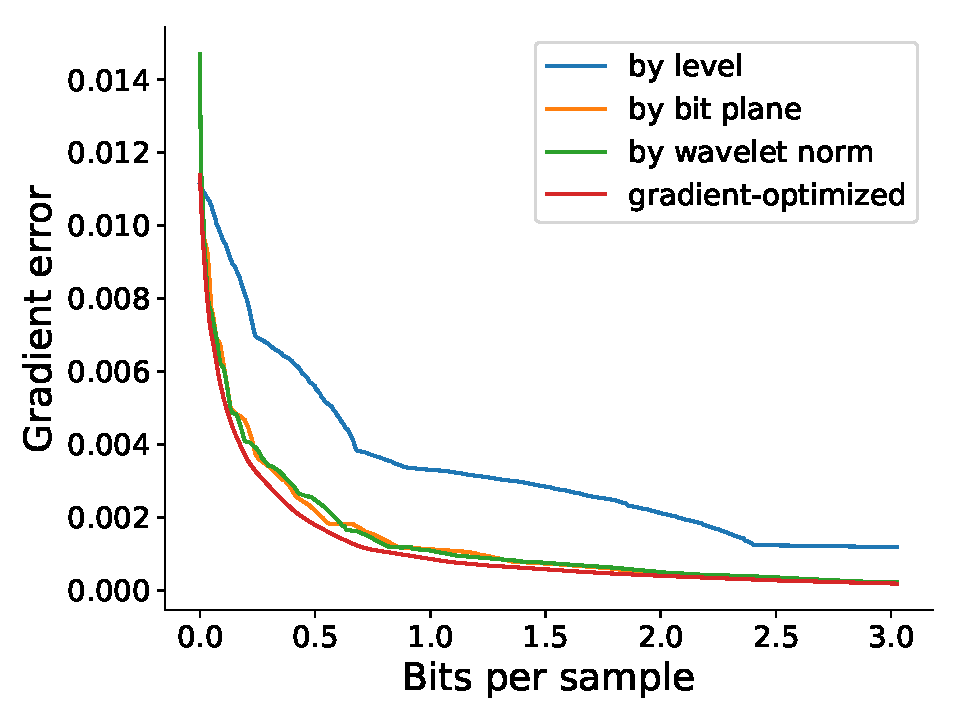
\includegraphics[width=0.48\linewidth]{gradient/gradient-optimized-diffusivity}}}
	\subcaptionbox{turbulence}{
	{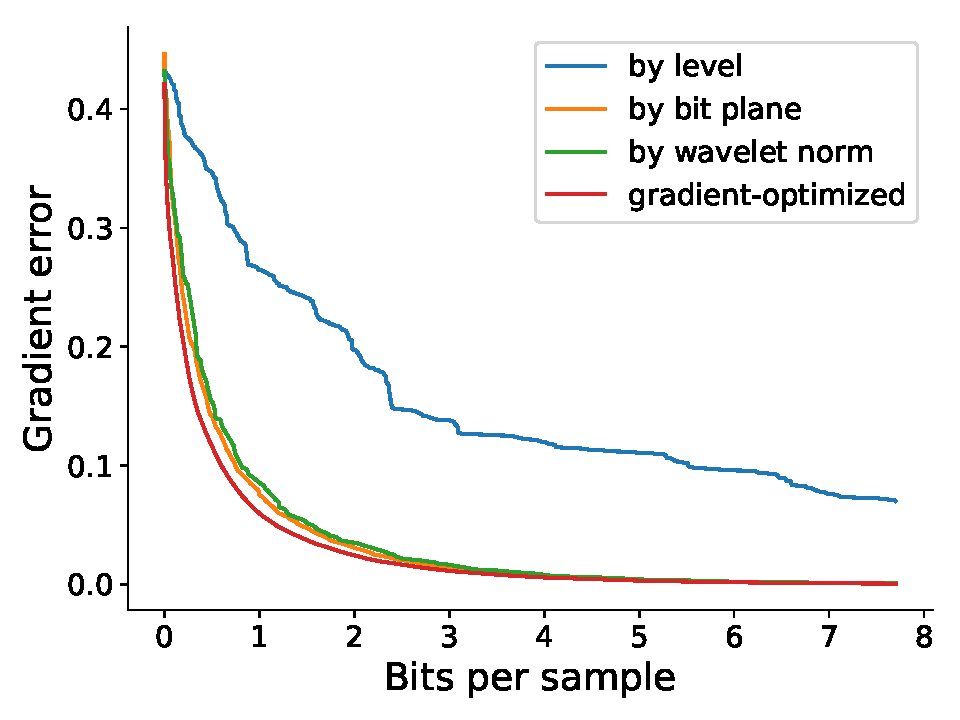
\includegraphics[width=0.48\linewidth]{gradient/gradient-optimized-turbulence}}}
	\subcaptionbox{pressure}{
	{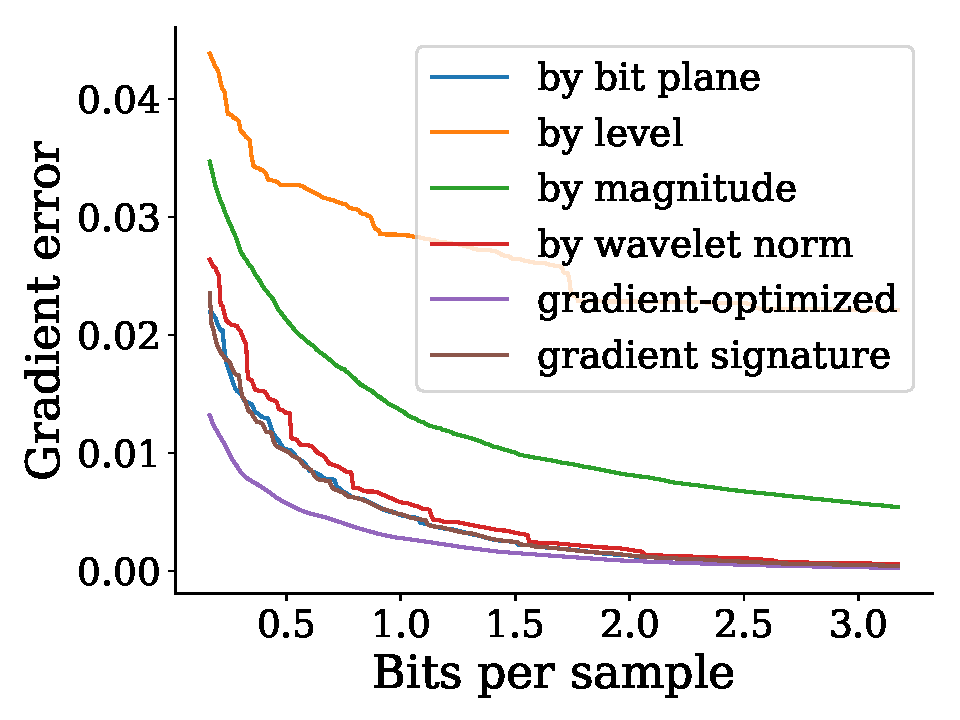
\includegraphics[width=0.48\linewidth]{gradient/gradient-optimized-pressure}}}
	% \subcaptionbox{marschner-lobb}{
	% {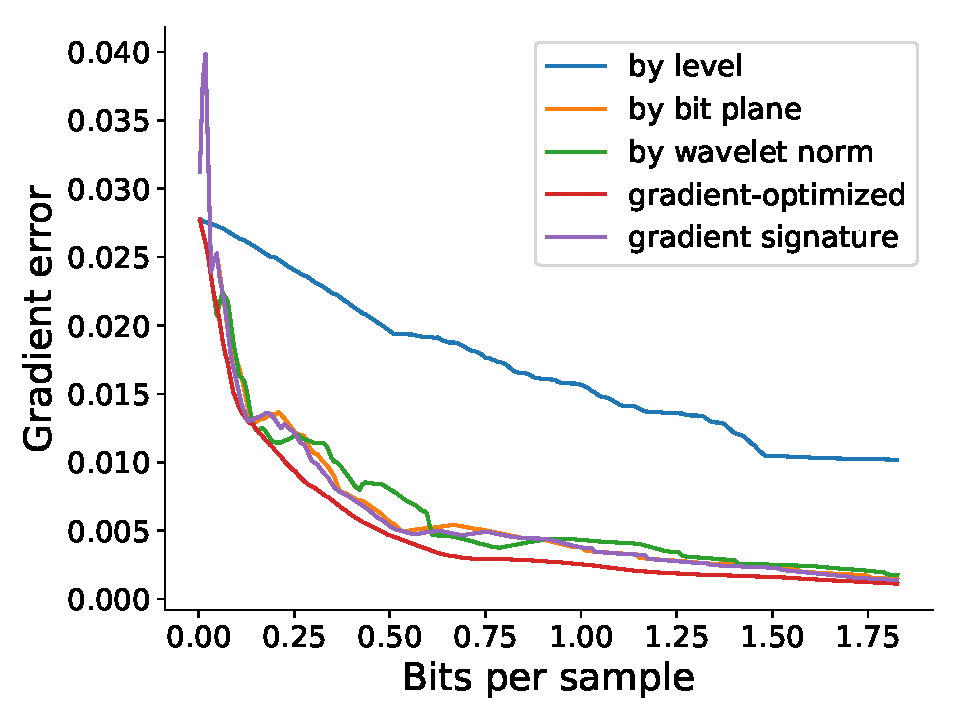
\includegraphics[width=0.48\linewidth]{img/gradient/5points/gradient-optimized-marschner-lobb.pdf}}}
	% \subcaptionbox{velocityz}{
	% {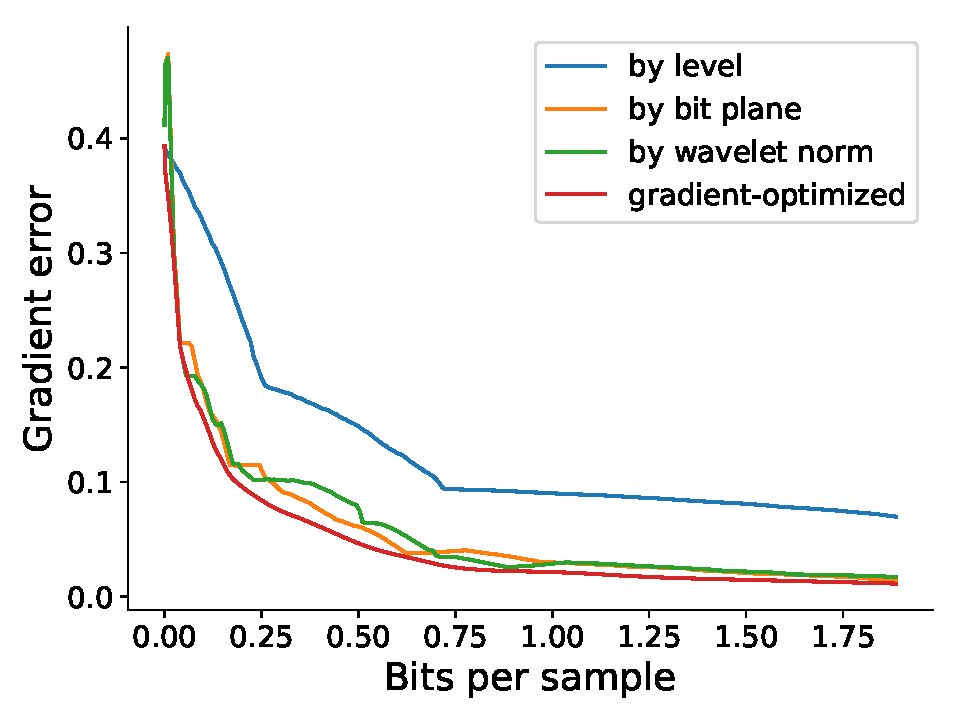
\includegraphics[width=0.48\linewidth]{img/gradient/5points/gradient-optimized-velocityz.pdf}}}
	\caption{Gradient error comparison among different streams, using the five-point stencil. The
	plots are truncated in the same way as in Figure \ref{fig:gradient-stencil-comparison}. In all
	cases, \emph{by wavelet norm} performs slightly worse than \emph{by bit plane} and \emph{gradient
	signature} do, but the differences are largely negligible. \emph{by level} performs the worst.}
	\label{fig:gradient-error-comparison}
\end{figure}

The differences in gradient errors among the \emph{by bit plane}, \emph{by wavelet norm}, and
\emph{gradient signature} streams are negligible. As an example, in
Figure~\ref{fig:gradient-rendering-diff} we visualize the three reconstructed gradient fields, as
well as the groundtruth gradient field for the \emph{velocityz} data set, at 0.35 bps, where the
streams diverge the most. This figure shows that the differences among reconstructed gradient fields
are barely visible. For this reason, in practice, any static stream would likely suffice for the
purpose of computing gradient. However, \emph{by bit plane} is significantly cheaper to compute
compared to \emph{gradient signature}, because the latter requires obtaining
\emph{gradient-optimized} first. \emph{by wavelet norm} is also a reasonable alternative, especially
if the bits are stored on disk in the same order, for example, to optimize for root-mean-square
errors (see Section~\ref{sec:motivation}. Finally, \emph{by wavelet norm} is also preferrable if,
beside an accurate gradient field, the task also requires an accurate function itself.

\begin{figure}[h]
	\centering
	\subcaptionbox{\emph{by level}}{
	{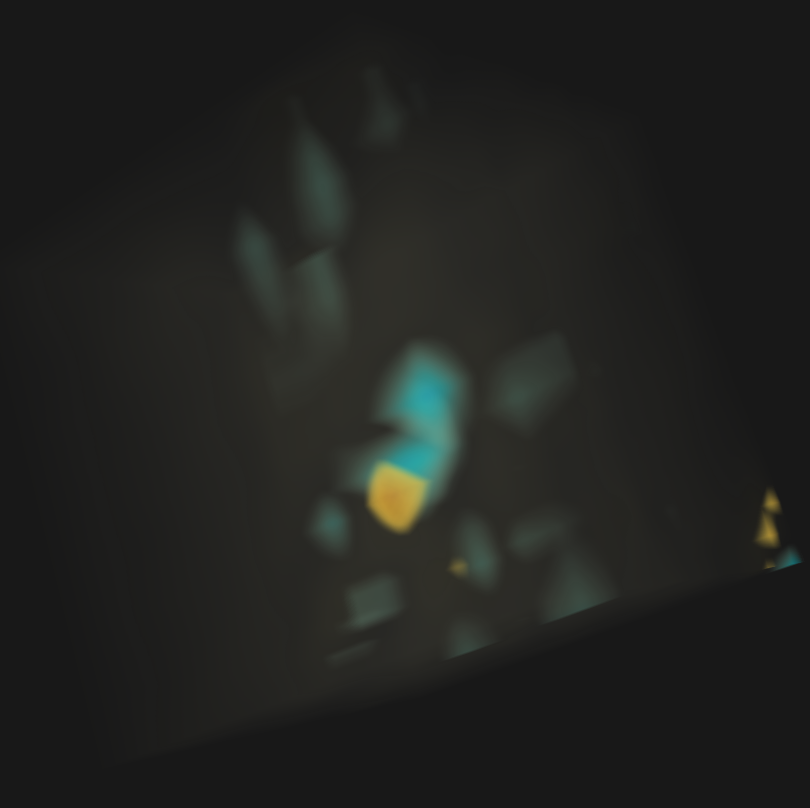
\includegraphics[width=0.31\linewidth]{gradient/gradient-turbulence-level}}}
	\subcaptionbox{\emph{by bit plane}}{
	{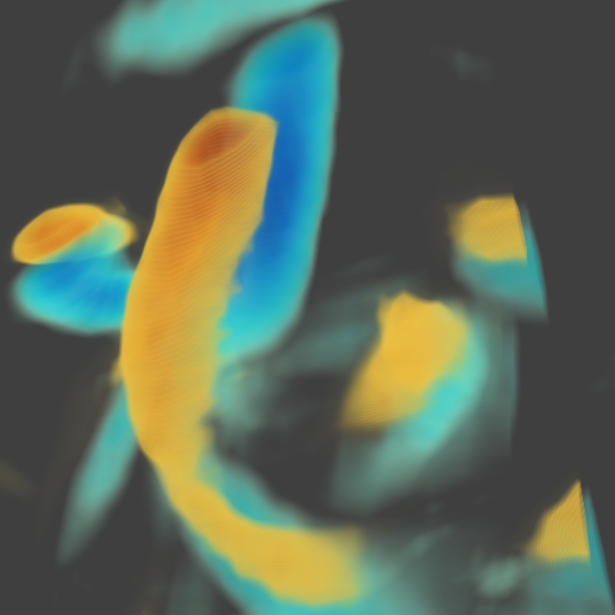
\includegraphics[width=0.31\linewidth]{gradient/gradient-turbulence-bit-plane}}}
	\subcaptionbox{\emph{by magnitude}}{
	{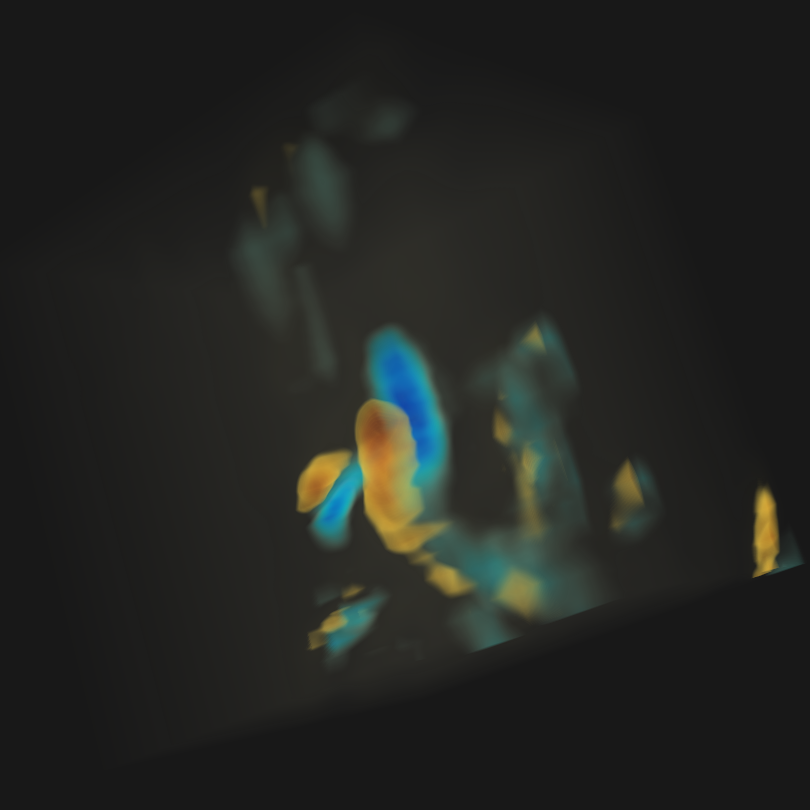
\includegraphics[width=0.31\linewidth]{gradient/gradient-turbulence-magnitude}}}
	\subcaptionbox{\emph{by wavelet norm}}{
	{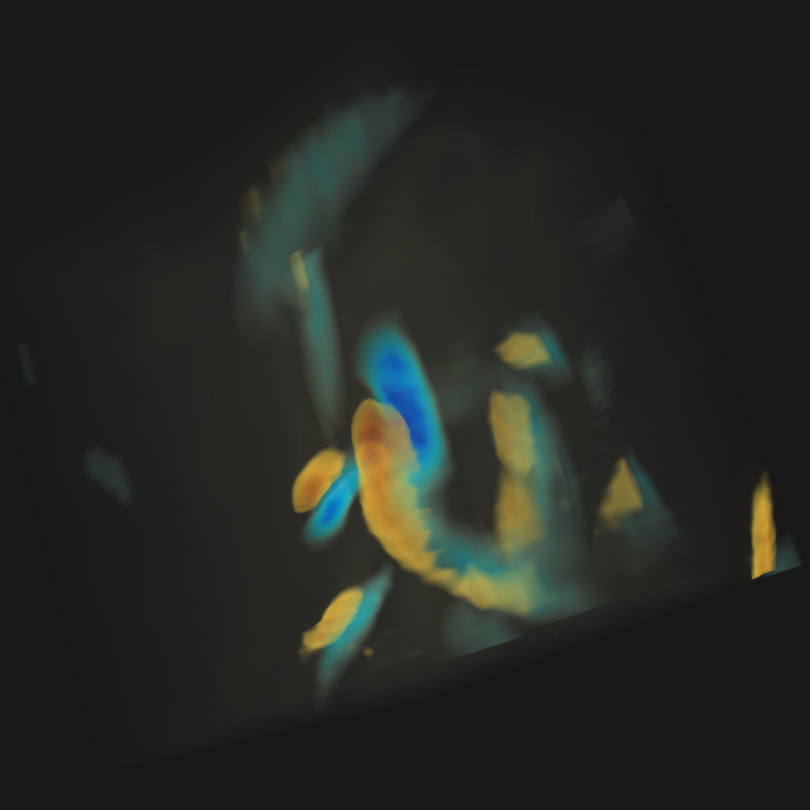
\includegraphics[width=0.31\linewidth]{gradient/gradient-turbulence-wavelet-norm}}}
	\subcaptionbox{\emph{by signature}}{
	{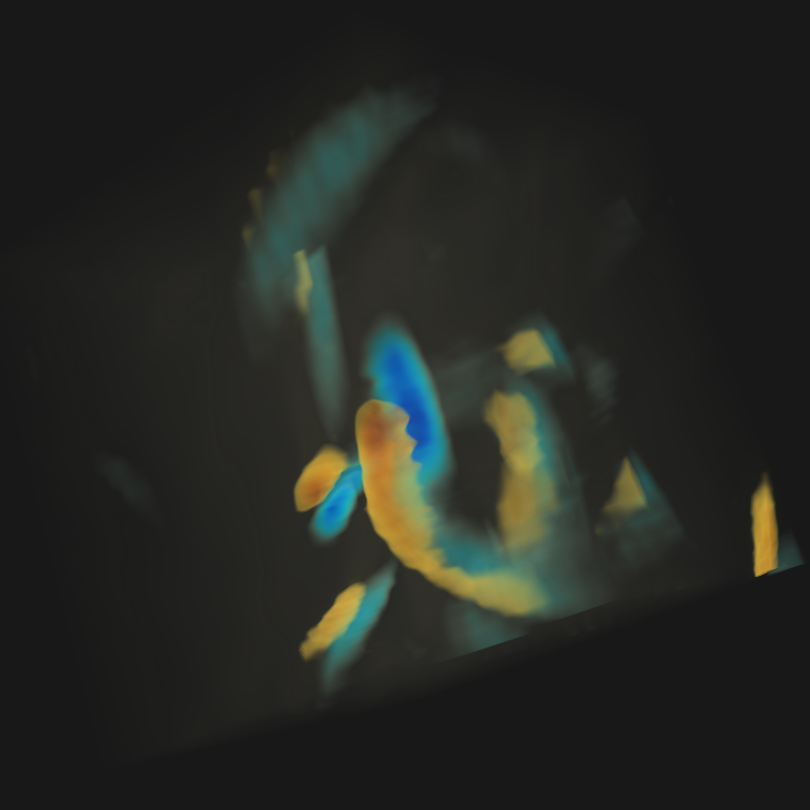
\includegraphics[width=0.31\linewidth]{gradient/gradient-turbulence-signature.png}}}
	\subcaptionbox{\emph{groundtruth}}{
	{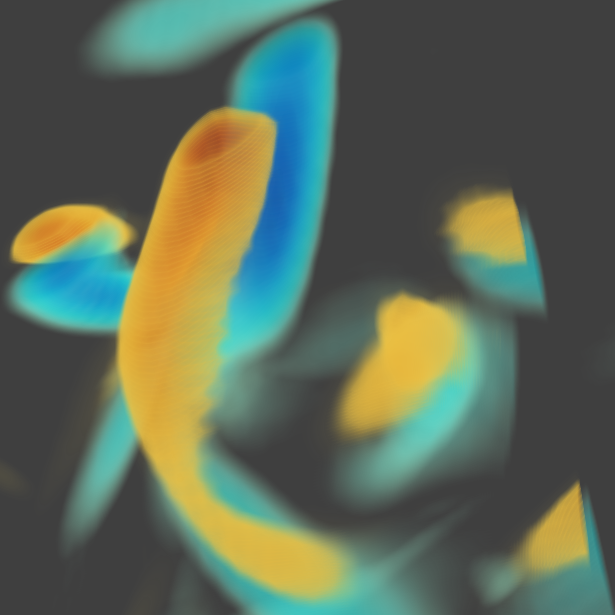
\includegraphics[width=0.31\linewidth]{gradient/gradient-turbulence-groundtruth.png}}}
	\caption{\emph{turbulence}, 0.2 bps}\label{fig:gradient-rendering-diff}
\end{figure}

Although \emph{gradient-optimized} and \emph{}

Figure~\ref{fig:gradient-renderings} gives a crude idea on the range of bit rates needed to
reconstruct a gradient field that is visually close to the ground-truth. For the data sets used in
our experiments, as low as 0.25 bps and as high as 2.39 bps are needed for this purpose.

\begin{figure}[h]
	\centering
	\subcaptionbox{\emph{by level}}{
	{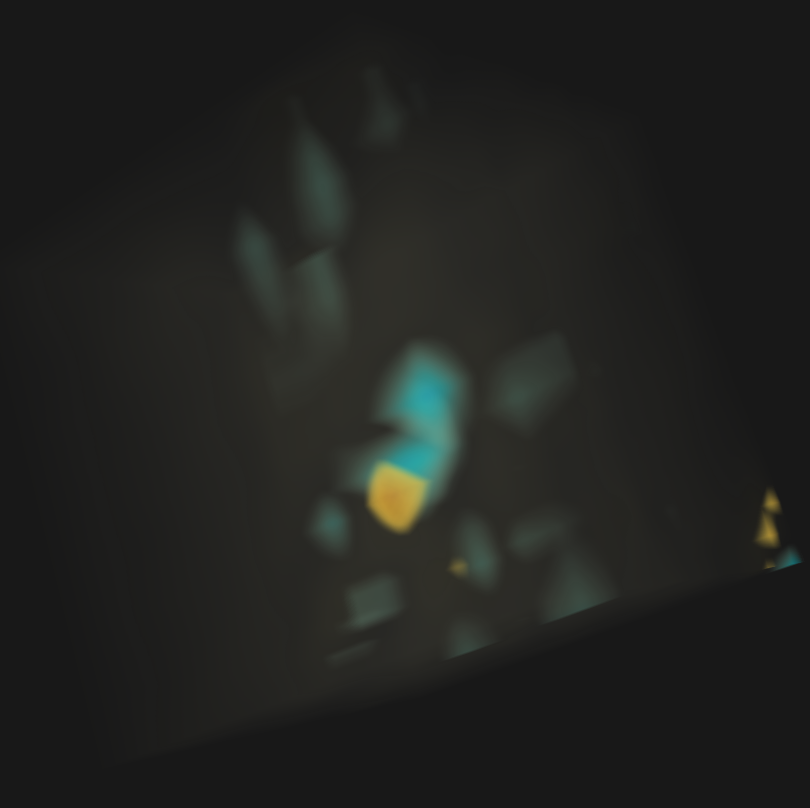
\includegraphics[width=0.31\linewidth]{gradient/gradient-turbulence-level}}}
	\subcaptionbox{\emph{by bit plane}}{
	{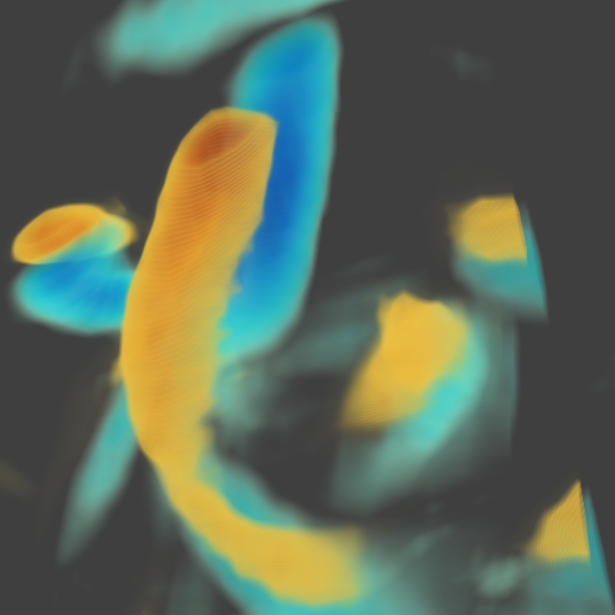
\includegraphics[width=0.31\linewidth]{gradient/gradient-turbulence-bit-plane}}}
	\subcaptionbox{\emph{by magnitude}}{
	{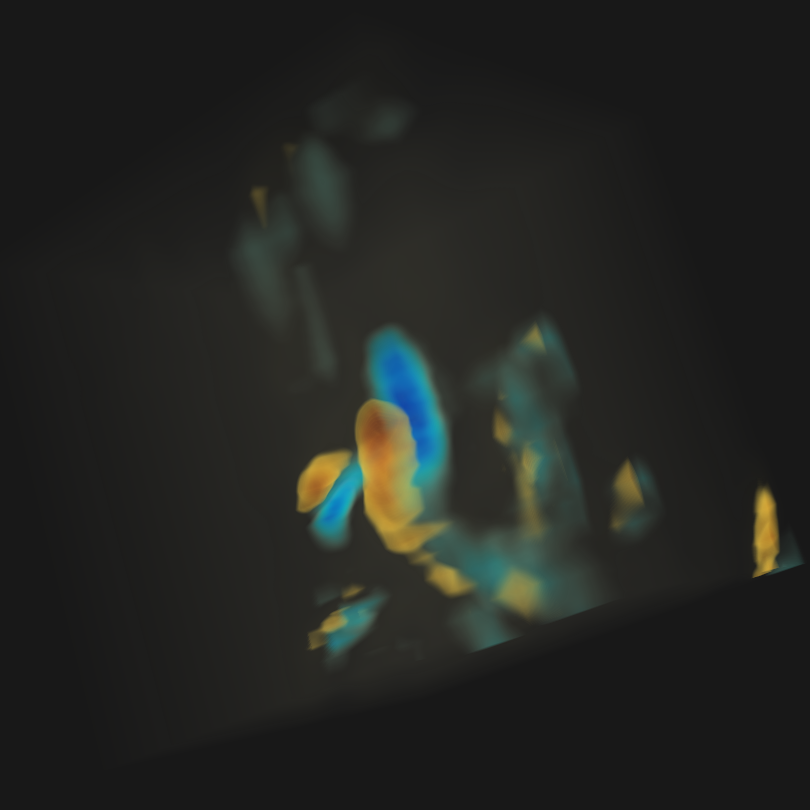
\includegraphics[width=0.31\linewidth]{gradient/gradient-turbulence-magnitude}}}
	\subcaptionbox{\emph{by wavelet norm}}{
	{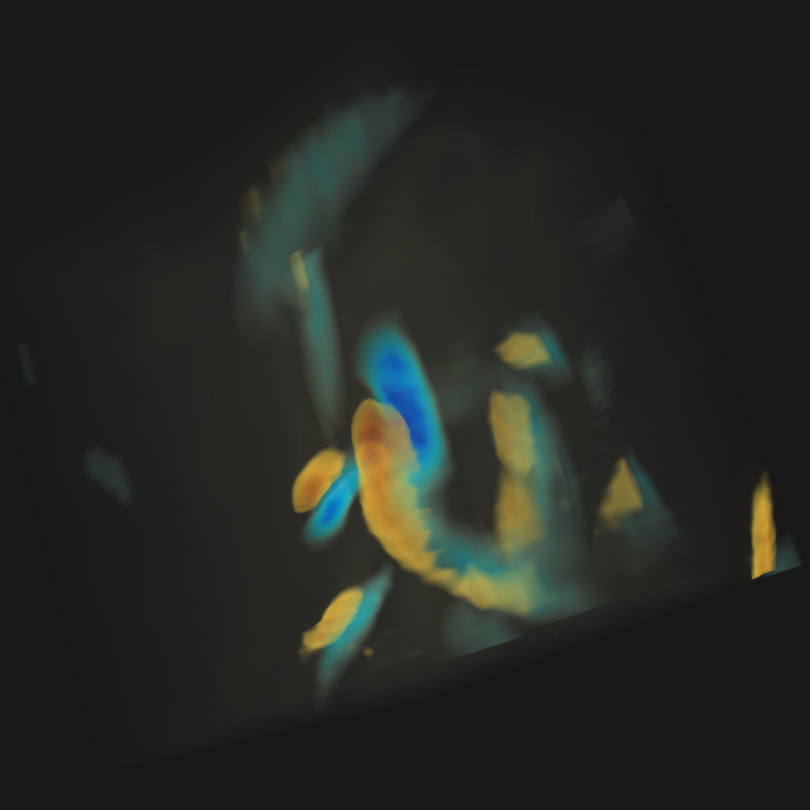
\includegraphics[width=0.31\linewidth]{gradient/gradient-turbulence-wavelet-norm}}}
	\subcaptionbox{\emph{by signature}}{
	{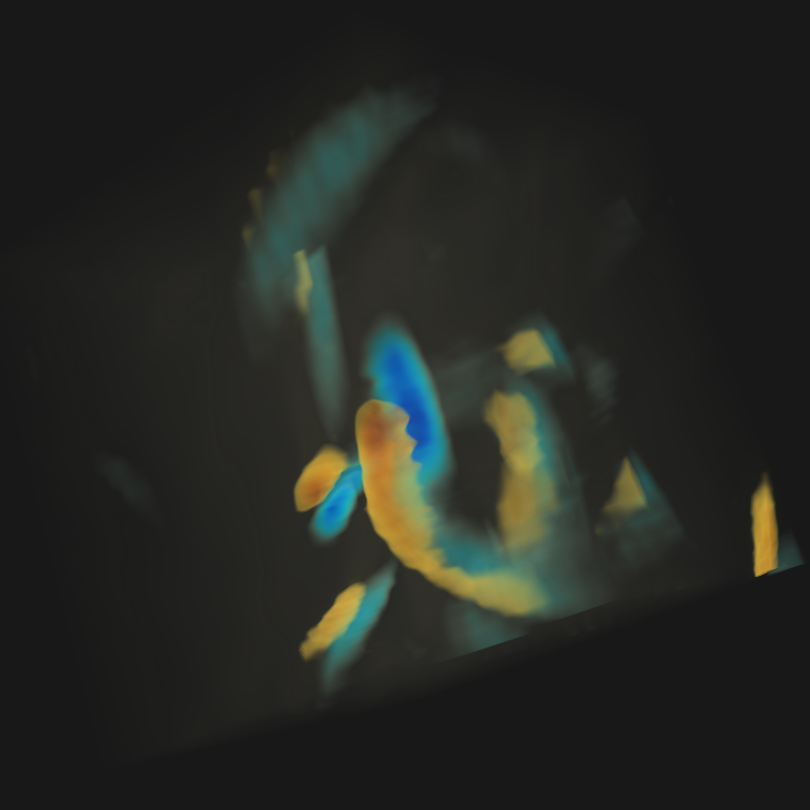
\includegraphics[width=0.31\linewidth]{gradient/gradient-turbulence-signature.png}}}
	\subcaptionbox{\emph{groundtruth}}{
	{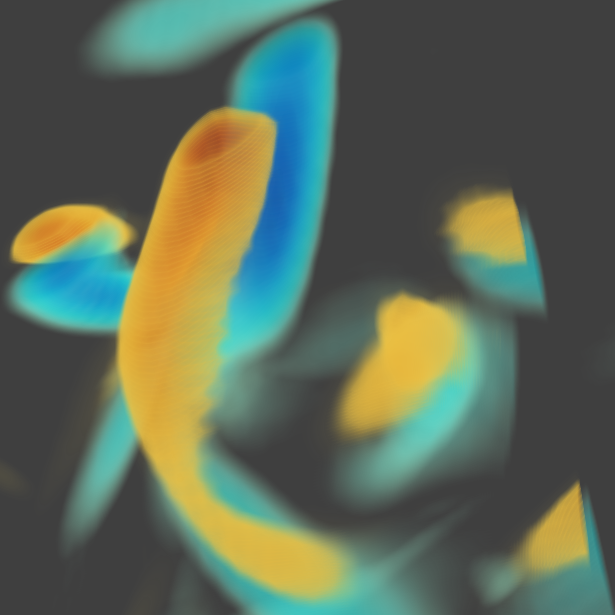
\includegraphics[width=0.31\linewidth]{gradient/gradient-turbulence-groundtruth.png}}}
	\caption{\emph{turbulence}, 0.2 bps}\label{fig:gradient-rendering-diff}
\end{figure}

\begin{figure}[h]
	\centering
	\subcaptionbox{\emph{by bit plane}}{
	{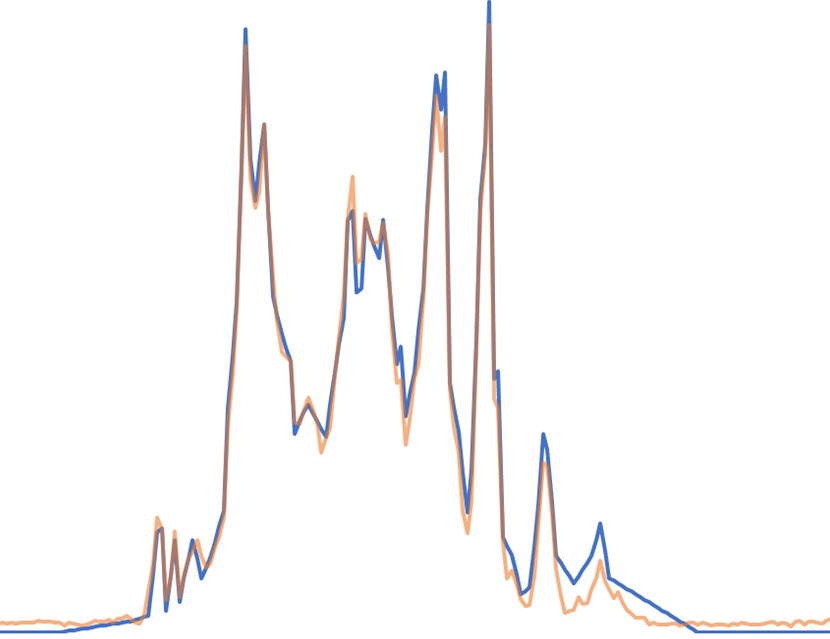
\includegraphics[width=0.31\linewidth]{gradient/gradient-bit-plane}}}
	\subcaptionbox{\emph{by	wavelet norm}}{
	{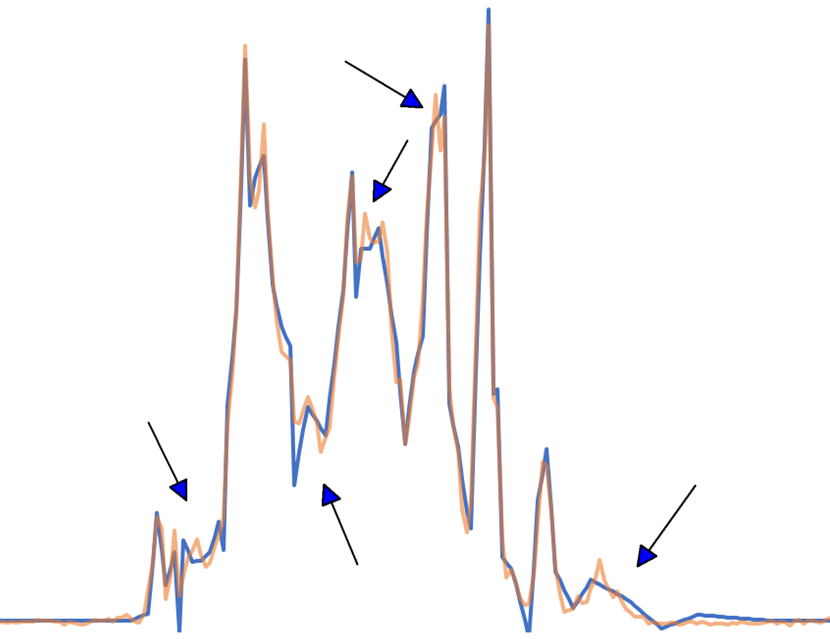
\includegraphics[width=0.31\linewidth]{gradient/gradient-wavelet-norm}}}
	\caption{\emph{turbulence}, 0.2 bps}\label{fig:gradient-rendering-diff}
\end{figure}

\subsubsection{Laplacian}\label{sec:laplacian}

The Laplace operator is a second-order differential operator, defined as the divergence of the
gradient field. It can be computed by summing second partial derivatives in all dimensions, for
example, in 2D: $\Delta f=(\frac{{\partial}^2}{\partial{x^2}}+\frac{{\partial}^2}{\partial{y^2}})f$.
To approximate the Laplacian for data on a grid, we use the three-point finite difference to
approximate the second derivative in each dimension: $\frac{{\partial}^2}{\partial{x^2}}f(x,y)
\approx f(x-1,y)-2f(x,y)+f(x+1,y)$. The Laplacian error is defined as the root-mean-square error
between the Laplacian of the reconstructed scalar field and the Laplacian of the original scalar
field, that is, $E_g(\Delta f_b,\Delta f)=RMSE(\Delta f_b,\Delta f)$. For each data set, Algorithm
[REF] is used to compute a \emph{laplacian-optimized} bit stream that minimizes $E_g$ at any bit
rate. From this stream, we obtain its signature and construct the \emph{laplacian signature} stream,
which, unlike \emph{laplacian-optimized}, is considered static and hence can be implemented in
practice. In Figure \ref{fig:laplacian-error-comparison} we compare these two stream against all the
previously defined streams, including \emph{gradient-optimized} using $E_g$ as the metric.

\begin{figure}[h]
	\centering
	\subcaptionbox{boiler}
	{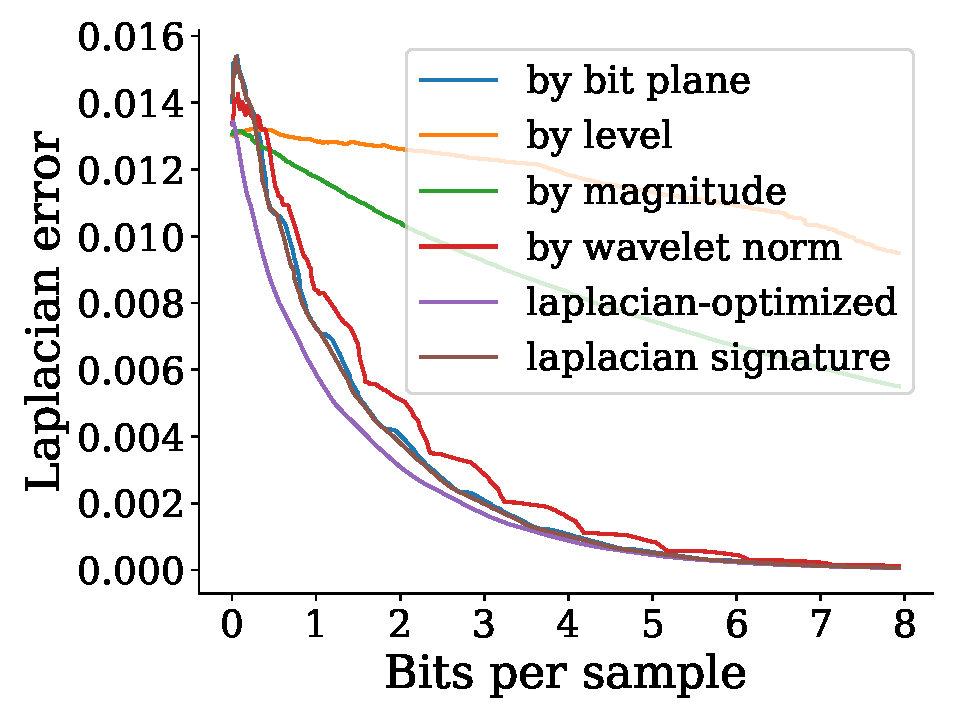
\includegraphics[width=0.48\linewidth]{laplacian/laplacian-optimized-boiler}}
	\subcaptionbox{diffusivity}
	{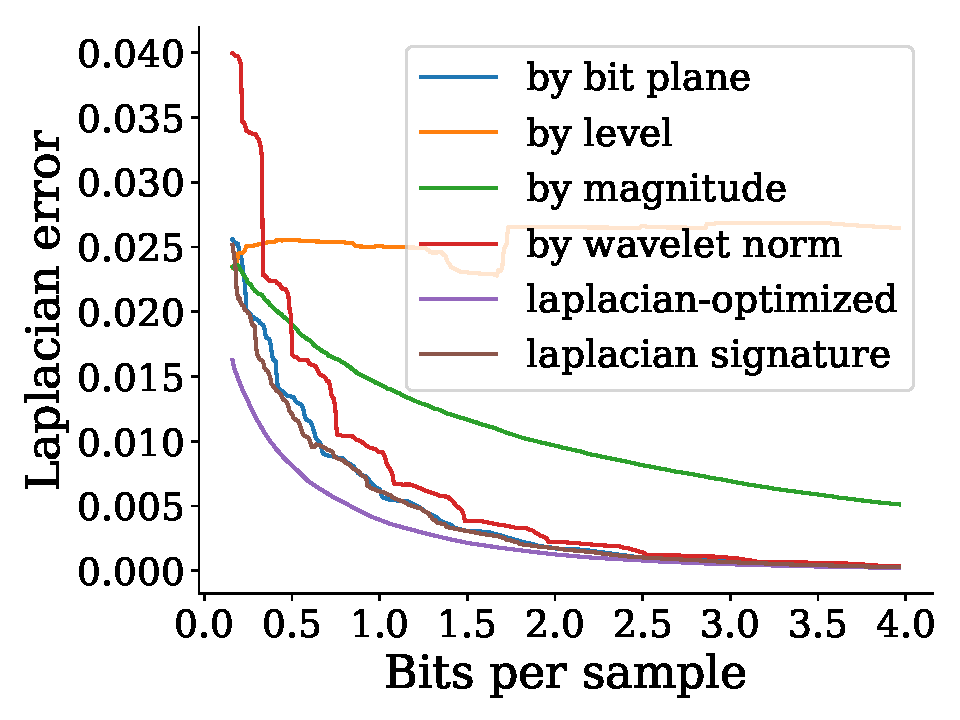
\includegraphics[width=0.48\linewidth]{laplacian/laplacian-optimized-diffusivity}}
	\subcaptionbox{turbulence}
	{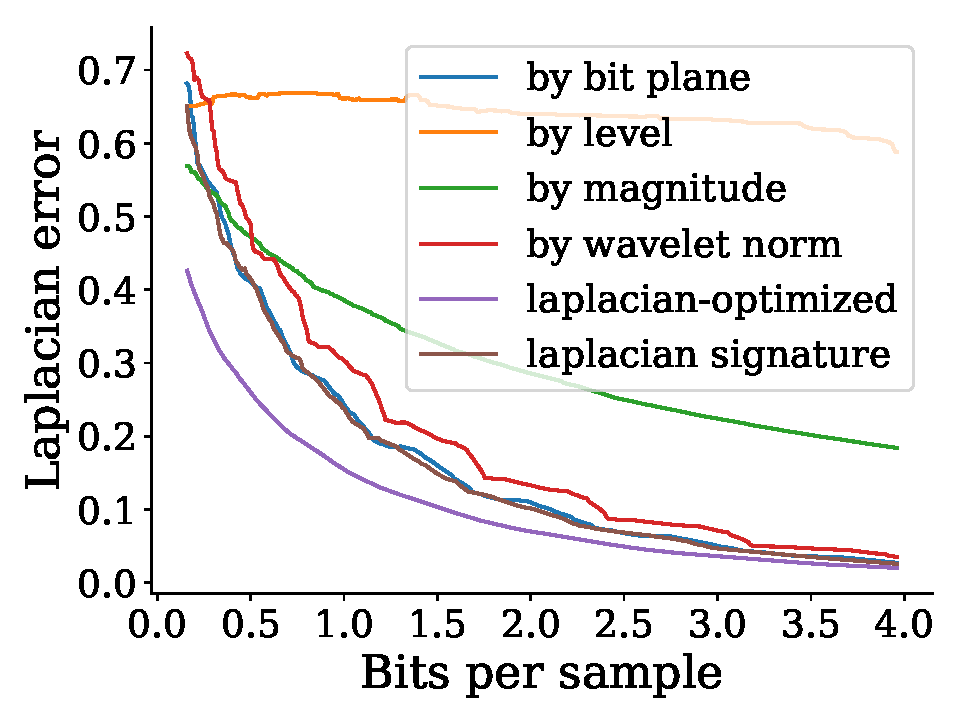
\includegraphics[width=0.48\linewidth]{laplacian/laplacian-optimized-turbulence}}
	\subcaptionbox{pressure}
	{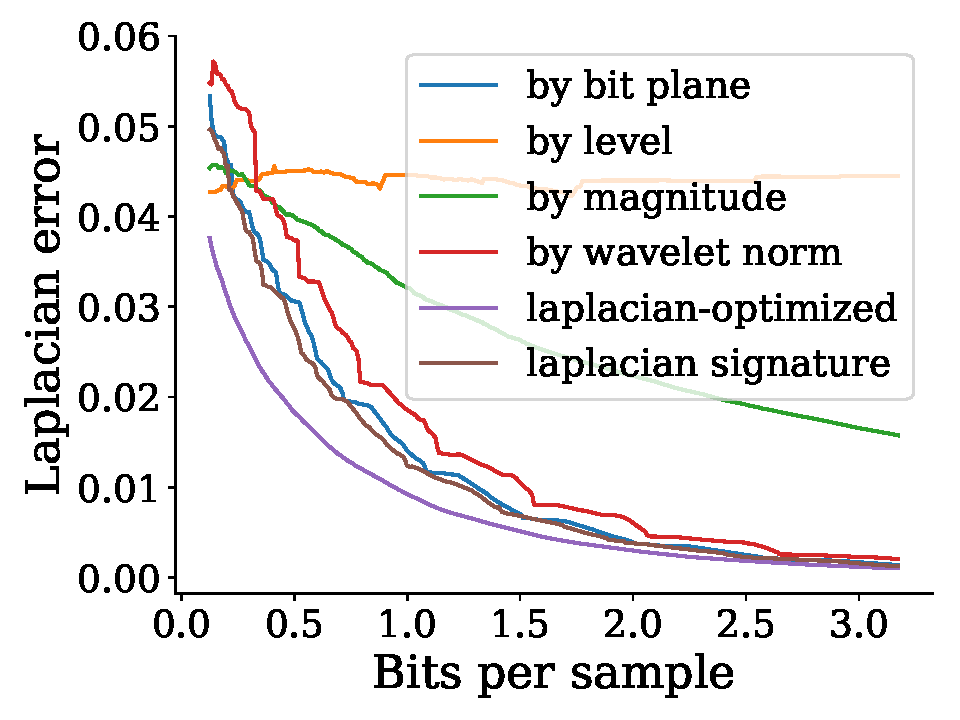
\includegraphics[width=0.48\linewidth]{laplacian/laplacian-optimized-pressure}}
	\caption{Laplacian error comparison among streams, using the three-point stencil. The plots are
	truncated so as to better highlight differences without discarding important information. In all cases, \emph{laplacian}}
	\label{fig:laplacian-error-comparison}
\end{figure}

It can be observed that unlike the case for gradient, there exists significant differences between
the \emph{rmse-optimized} and \emph{laplacian-optimized} streams with regards. To understand these
differences we plot the precision of every wavelet coefficients at a low bit rate in Figure
\ref{fig:laplacian-precision-comparison} (a and b). When cross refererencing this Figure with Figure
\ref{fig:gradient-comparison}b we see that the \emph{laplacian-optimized} stream priotizes
finer-resolution bits where the sharp shockwave is, unlike the \emph{rmse-optimized} stream which
prefers lower-ordered, coarse-resolution bits. This effect makes sense intuitively, as the
derivative operator makes functions less smooth, hence amplifing hard edges. This happens in the
gradient case too, but to a much lesser degree.

\begin{figure}[h]
	\centering
	\subcaptionbox{\emph{by level}}
	{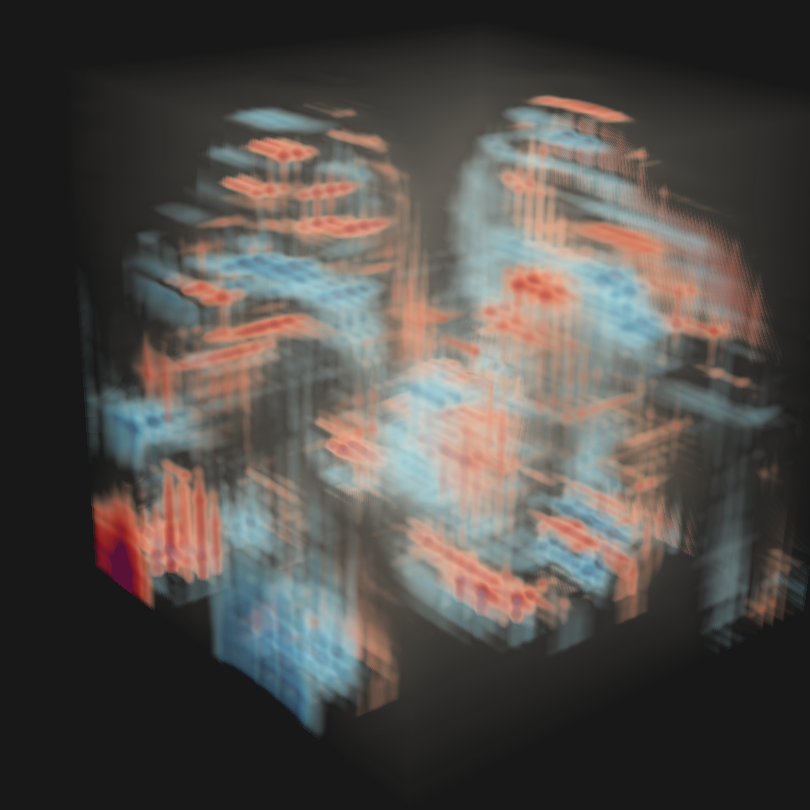
\includegraphics[width=0.31\linewidth]{laplacian/laplacian-pressure-level}}
	\subcaptionbox{\emph{by bit plane}}
	{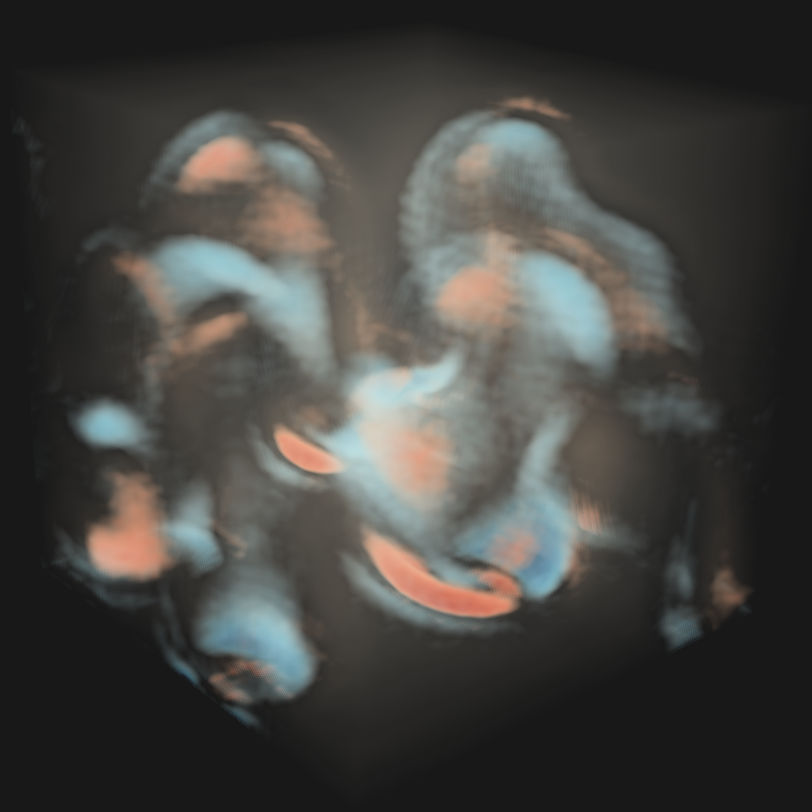
\includegraphics[width=0.31\linewidth]{laplacian/laplacian-pressure-bit-plane}}
	\subcaptionbox{\emph{by magnitude}}
	{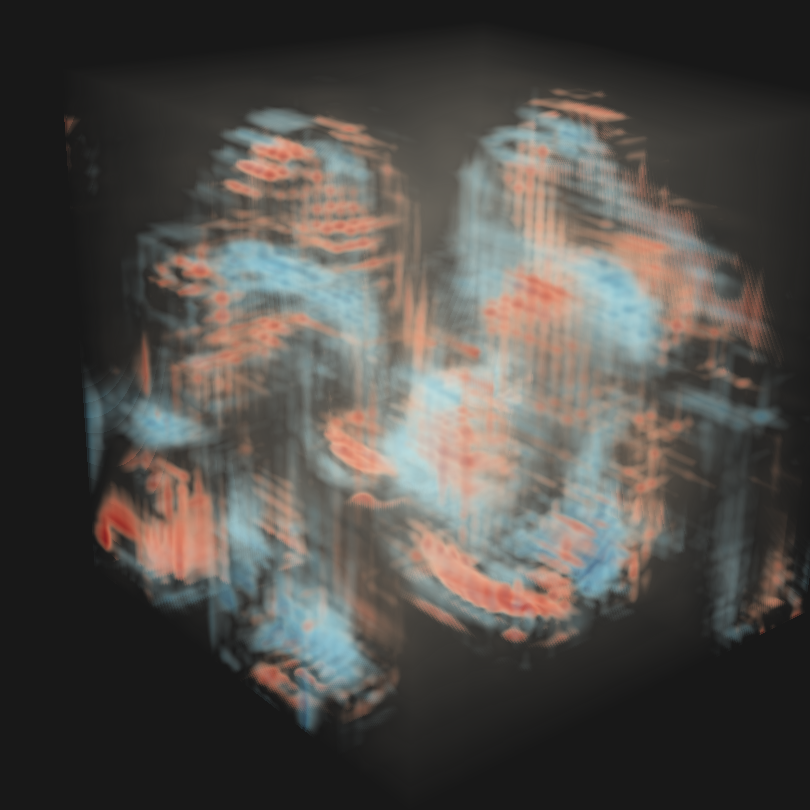
\includegraphics[width=0.31\linewidth]{laplacian/laplacian-pressure-magnitude}}
	\subcaptionbox{\emph{by wavelet norm}}
	{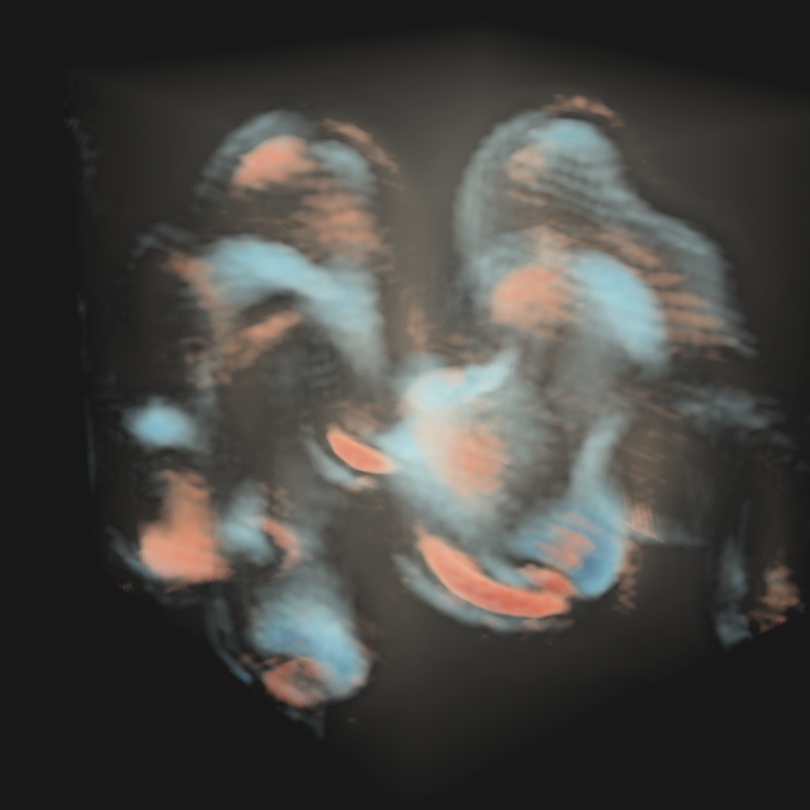
\includegraphics[width=0.31\linewidth]{laplacian/laplacian-pressure-wavelet-norm}}
	\subcaptionbox{\emph{by signature}}
	{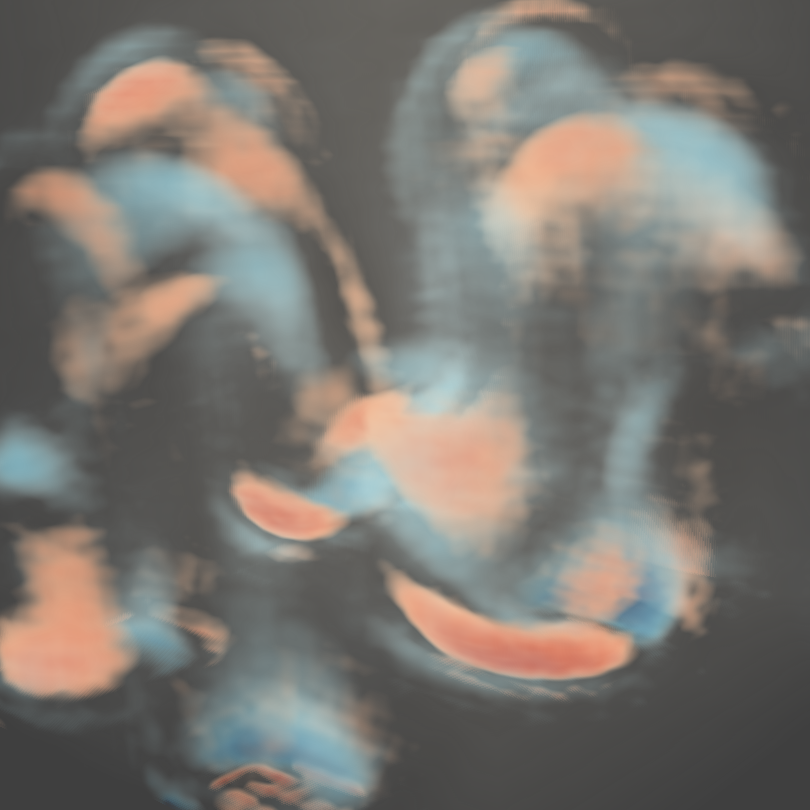
\includegraphics[width=0.31\linewidth]{laplacian/laplacian-pressure-signature}}
	\subcaptionbox{\emph{groundtruth}}
	{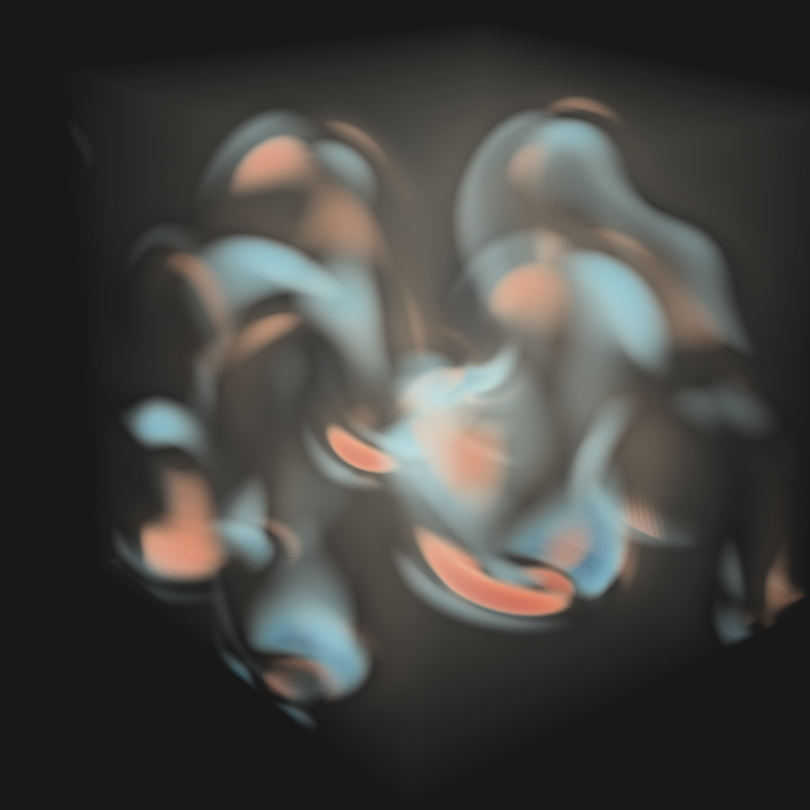
\includegraphics[width=0.31\linewidth]{laplacian/laplacian-pressure-groundtruth}}
	\caption{pressure, laplacian, 0.9 bps}
	\label{fig:laplacian-precision-comparison}
\end{figure}

\begin{figure}[h]
	\subcaptionbox{\emph{by wavelet norm}}
	{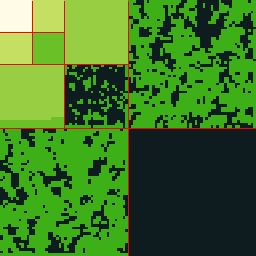
\includegraphics[width=0.32\linewidth]{img/laplacian/by-wavelet-norm.png}}
	\subcaptionbox{\emph{by bit plane}}
	{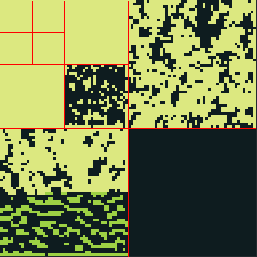
\includegraphics[width=0.32\linewidth]{img/laplacian/by-bit-plane.png}}
	\subcaptionbox{\emph{laplacian signature}}
	{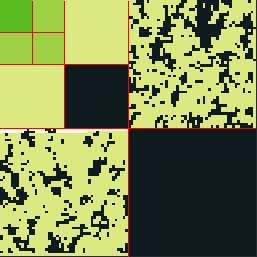
\includegraphics[width=0.32\linewidth]{img/laplacian/laplacian-signature.png}}
	\subcaptionbox{\emph{laplacian-optimized}}
	{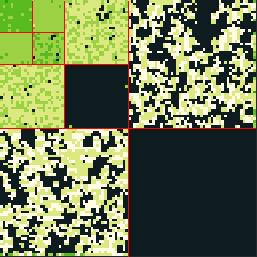
\includegraphics[width=0.32\linewidth]{img/laplacian/laplacian-optimized.png}}
	\subcaptionbox{\emph{gradient signature}}
	{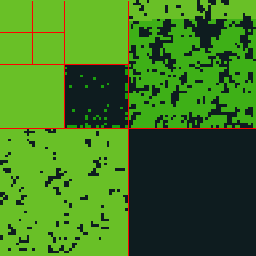
\includegraphics[width=0.32\linewidth]{img/laplacian/gradient-signature.png}}
	\caption{Precision map per subband (brigther is more precise) \emph{velocityz}, 1.28 bps. \emph{by wavelet norm} allocates more bits for the coarse-level subbands, while \emph{laplacian-optimized} and \emph{laplacian signature} do the opposite.}
	\label{fig:laplacian-precision-comparison}
\end{figure}

\emph{rmse-optimized}, \emph{laplacian-optimized}, and also \emph{gradient-optimized} for the euler
data set are visualized in Figure \ref{fig:signature-comparison}. 

TODO: add comparison of stream signatures
% \begin{figure}[h]
% 	\centering
% 	\subcaptionbox{\emph{rmse-optimized}}
% 	{
\includegraphics[width=0.32\linewidth]{img/gradient-laplacian/SIG-GREEDY-(rmse).png}}
% 	\subcaptionbox{\emph{laplacian-optimized}}
% 	{
\includegraphics[width=0.32\linewidth]{img/gradient-laplacian/SIG-GREEDY-(laplacian).png}}
% 	\subcaptionbox{\emph{gradient-optimized}}
% 	{
\includegraphics[width=0.32\linewidth]{img/gradient-laplacian/SIG-GREEDY-(gradient).png}}
% 	\caption{Stream signatures visualized through a linear-blue color map (brighter is higher
% 	priority). From left to right: higher-ordered to lower-ordered bit planes. From top to bottom:
% 	coarser to finer subbands. Note that the streams from which the signatures are extracted do not
% 	contain leading zero bits, which explains the very dark cells }
% 	\label{fig:signature-comparison}
% \end{figure}

Using the signature for \emph{laplacian-optimized}, we are able construct a data-independent stream
(in the sense that once the signature is computed and is given, the ordering of the bits follows the
the signature only). This stream, called \emph{laplacian signature}, performs at least as well as,
and often better, than \emph{rmse-optimized} for all data sets (see Figure
\ref{fig:laplacian-comparison}). The reason \emph{laplacian signature} does not always outperform
\emph{rmse-optimized}, and that there is still a gap between itself and \emph{laplacian-optimized}
is that the signature is computed essentially by `'averaging'' local signatures, a process that
lessen the effectiveness of the signature when the data is highly inhomogenous (e.g., the euler data
set with its sharp shockwaves). Nevertheless, even with one signature for the whole domain, we are
able to reconstruct more accurate Laplacian in all cases in experiment. In practice, the signature
is a tiny piece of meta information that can be pre-computed, stored, and transmitted before any
value bits to help `'steer'' the data stream, whenever Laplacian is the quantity of interest.
